\documentclass[linenumber]{jdsart}

\volume{0}
\issue{0}
\pubyear{2022}
\articletype{research-article}
\doi{0000}

\usepackage{siunitx} % For alignment of numbers
\sisetup{
    group-separator = {,},
    round-mode = places,
    round-precision = 2,
    output-decimal-marker = {.},
    table-number-alignment = center,
    table-figures-integer = 6,
    table-figures-decimal = 2,
    table-figures-uncertainty = 2
}

% image path
\graphicspath{{.}{./images}}

\usepackage{xcolor}
\newcommand{\dt}[1]{\textcolor{purple}{DT: (#1)}}
\newcommand{\jy}[1]{\textcolor{cyan}{JY: (#1)}}

\let\proglang=\textsf
%% \newcommand{\pkg}[1]{{\fontseries{m}\selectfont #1}}
%% \newcommand\code[2][black]{\textcolor{#1}{\texttt{#2}}}

\usepackage{comment}
\usepackage{booktabs, textgreek}

%% float control
\renewcommand\floatpagefraction{0.75}
% \renewcommand\topfraction{.8}
% \renewcommand\bottomfraction{.8}
% \renewcommand\textfraction{.2}
\setcounter{totalnumber}{50}
\setcounter{topnumber}{50}
\setcounter{bottomnumber}{50}

\begin{document}

\begin{frontmatter}
  
\title{Principles for Open Data Curation: A Case Study with the New
York City 311 Service Request Data}
\runtitle{Principles for Open Data Curation}

\author[1]{\inits{D.}\fnms{David}~\snm{Tussey}}
\author[2]{\inits{J.}\fnms{Jun}~\snm{Yan}}
\address[1]{\institution{NYC DoITT}, \cny{USA}}
\address[2]{Department of Statistics,
  \institution{University of Connecticut}, \cny{USA}}



 \tableofcontents % Optional: Table of Contents
 \listoffigures % List of Figures
 \listoftables % List of Tables

\hyphenpenalty=750

\begin{abstract}
In the early 21st century, the open data movement began to transform 
societies and governments by promoting transparency,
innovation, and public engagement. New York City (NYC) has been at
the forefront of this movement since the enactment of the Open 
Data Law in 2012, which led to the creation of the NYC Open Data
portal. This portal now hosts 2,700 datasets from 80 city agencies,
serving as a crucial resource for research across various domains, 
including health, urban development, and transportation. The 
success of these initiatives highlights the importance of data 
curation in ensuring the utility and reliability of open datasets.
This paper examines the challenges of open data curation through a
case study of the NYC 311 Service Request (SR), addressing issues 
of data validity, consistency, and curation efficiency. Based on 
insights from this case study, we propose a set of data curation 
principles tailored for government-released open data. These principles 
aim to enhance data management practices and ensure 
the ongoing utility of open data. The paper concludes with 
actionable recommendations for enhancing data curation and outlines
general principles for the effective release of open data.

\end{abstract}

\begin{keywords}
  \kwd{Data cleansing}
  \kwd{Data Curation}
  \kwd{Data science}
  \kwd{NYC Open Data}
  \kwd{Open data}
  \kwd{Smart Cities}
  \kwd{Transparency}
\end{keywords}

\end{frontmatter}

\section{INTRODUCTION} 
\label{sec:intro}

In the early 21st century, the open data movement began 
to take shape, driven by the fundamental belief that 
freely accessible data can transform both societies and 
governments. This movement champions the principles
of transparency, innovation, and public engagement. 
A landmark in this journey was the launch of the United States'
\href{https://www.data.gov}{Data.gov} portal in 2009, a pioneering
platform in making government data widely accessible. Shortly after,
the European Union followed suit, unveiling its
\href{https://data.europa.eu/euodp}{Open Data Portal} in 2012, further
cementing the movement's global reach. Furthermore, the World Bank's Open
Data initiative, initiated in 2010, stands out as a comprehensive
repository for global development data, available at
\href{https://data.worldbank.org}{World Bank Open Data}. 
These initiatives represent significant strides in democratizing data, 
in breaking barriers that once kept valuable information 
on government performance in silos. Their collective impact 
is profound, extending beyond mere data sharing to 
fostering a culture of openness that benefits individuals, 
communities, governments, and economies worldwide 
\citep{barns2016mine, wang2016adoption}.


New York City (NYC) has emerged as a leader in the open data movement,
marked by the enactment of the Open Data Law in 2012
\citep{zuiderwijk2014open}. This landmark legislation led to the
creation of the \href{https://opendata.cityofnewyork.us}{NYC Open Data
  portal}, which today hosts an impressive array of 2,700 datasets
from 80 different city agencies. This resource has become invaluable
for researchers across various fields and has significantly enhanced
local government transparency. Popular datasets include information on
restaurant health inspection violations, car crashes, high school and
college enrollment statistics, jail inmate charges, and the location
of city-wide free Internet access points. These datasets have been
applied in civil life in various ways, such as mapping car crashes
involving pedestrians and visualizing high school and college
enrollment trends. Furthermore, they have enabled significant research
across multiple domains, including health \citep{cantor2018facets,
  shankar2021data}, urban development \citep{neves2020impacts}, and
transportation \citep{gerte2019understanding}, aiding in the
understanding and addressing of complex urban challenges.


The civil and research applications of open data critically depend on
its quality, making data curation fundamental in the open data
ecosystem. Among the earliest discussions,
\citet{witt2009constructing} focused on developing data curation
profiles tailored to specific contexts, setting a precedent for
targeted data management strategies. Addressing broader challenges in
data sharing and management, \citet{borgman2012conundrum} highlighted
the complexities of research data distribution, emphasizing the need
for robust strategies. This is complemented by \citet{hart2016ten},
who outlined essential principles for effective data management,
particularly emphasizing meticulous curation practices. In
collaborative data management, \citet{beheshti2019datasynapse}
underscored the significance of cooperative environments for managing
and sharing social data effectively. This aspect gains further
relevance in \citet{mclure2014data}, which delved into the specific
practices and needs within data curation communities. The practical
implications of data curation are vividly illustrated in public health
and global challenges. \citet{cantor2018facets} demonstrated the
utility of curated open data in evaluating community health
determinants. The COVID-19 pandemic served as a real-world example,
with \citet{shankar2021data} observing the critical role of collective
data curation efforts in managing and responding to the
crisis. Collectively, these studies highlight the multifaceted nature
of data curation and emphasize its indispensable role in enhancing the
applicability and value of open data across various domains.


The contributions of this paper are twofold. First, we delve into
the specifics of data curation challenges using the NYC 311 Service
Request (SR) Data as a case study. This renowned and frequently viewed 
dataset serves as a prime example for examining key issues in data curation, 
including data validity, consistency, and curation efficiency. 
We illustrate these points with live examples drawn from our 
processing of the 311 SR data. Secondly, building upon insights 
gained from this case study, we propose a set of data curation 
principles tailored for government-released open data. These 
principles are designed to address the unique challenges 
and requirements observed in the curation of such datasets.

\jy{How about putting all these sections into one section on case
  study? They can be subsections in the merged section.
  After that, we can have a section on recommendations for open
  data curation based on what we learn from the case study. For each
  recommended principle, we can link to the specifics of the case
  study.}

The paper is organized as follows:
Section~\ref{sec:data} `\textit{NYC 31 Service Request Data} offers a 
look at the history of the 311system. Long-term trends are 
presented in a 10-year data analysis (2014-2023).
Section~\ref{sec:issues} \textit{Data Cleansing Issues} offers a 
discussion of specific data cleansing issues impacting data quality and 
curation efficiency. These issues include structural issues, compliance 
with the Data Dictionary, and missing, blank, or N/A entries. We also
explore field compliance with a domain of legal or acceptable values.
Next we deal with several important issues surrounding logical inconsistencies 
and concerning patterns found in the data. We also explore an issue of precision 
versus accuracy. This section concludes by identifying duplicate/redundant data fields
and Data Dictionary observation. Section~\ref{sec:recommendations} 
\textit{Recommendations} provides actionable suggestions for 
mitigating or resolving the identified issues. Section~\ref{sec:discussion} ``Discussions'' 
concludes with an encapsulation of key insights and implications of our research.


\section{NYC 311 Service Request Data} 
\label{sec:data}
The NYC 311 service, a critical component of New York City's public
engagement and service response framework, serves as a centralized hub
for non-emergency inquiries and requests. Introduced in 2003, the NYC
311 system was designed to streamline the city's response to
non-emergency issues, ranging from noise complaints to street
maintenance requests. Initially a phone-based call center, the system
evolved into a comprehensive data management platform handling
millions of requests annually. Key milestones since its launch in 2003
include the addition of online and mobile app channels in 2009, a
record high of 348,463 monthly service requests in August 2020 due to
the COVID-19 pandemic, the 2021 expansion to include the MTA's city
subway system, and a record 3.23 million service requests in
2023. Today, the NYC 311 data system manages over 3 million service
requests per year. This data is publicly accessible through the NYC Open Data
Portal, which provides tools for querying, grouping, aggregating,
geo-mapping, visualizing, and exporting results. The
\href{https://www.nyc.gov/content/oti/pages/}{NYC Office of Technology
  and Innovation (OTI)}, which provides technological support for the
open data system. 

\begin{comment}
Despite its success, the 311 system faces several challenges:
data timeliness, accuracy, and consistency, difficulties in
correlating data over long periods, excluding personally
identifiable information (PII), integration with stand-alone systems
at selected NYC agencies, and managing API usagefor numerous
third-party users. These challenges are addressed by various agency
open data managers and 
\end{comment}

The impact of NYC 311 data extends beyond operational efficiency; it
has become instrumental in shaping city governance and community
engagement. This open data not only ensures governmental transparency
but also empowers researchers, civic developers, and the general
public. The data has been pivotal in providing advice on shelters
during emergencies, handling inquiries during the COVID-19 pandemic,
enforcing standards between landlords and tenants, reallocating taxi
routes based on analyses by the Taxi and Limousine Commission (TLC),
and improving responsiveness across City Agencies

To begin, we looked at a 10-year period (2014-2023) to
observe a longer time-frame; see
Figure~\ref{fig:10-yr-monthly}. During that time-frame,
the number of 311 SRs grew by nearly 50\%.


\jy{The 'title' in each figure could be removed because we have
  captions. The fonts of the annotations in the figures need to be
  increased. The code generating them need to be tidied for future
  sharing.
}



\begin{figure}[tbp]
	\centering
  	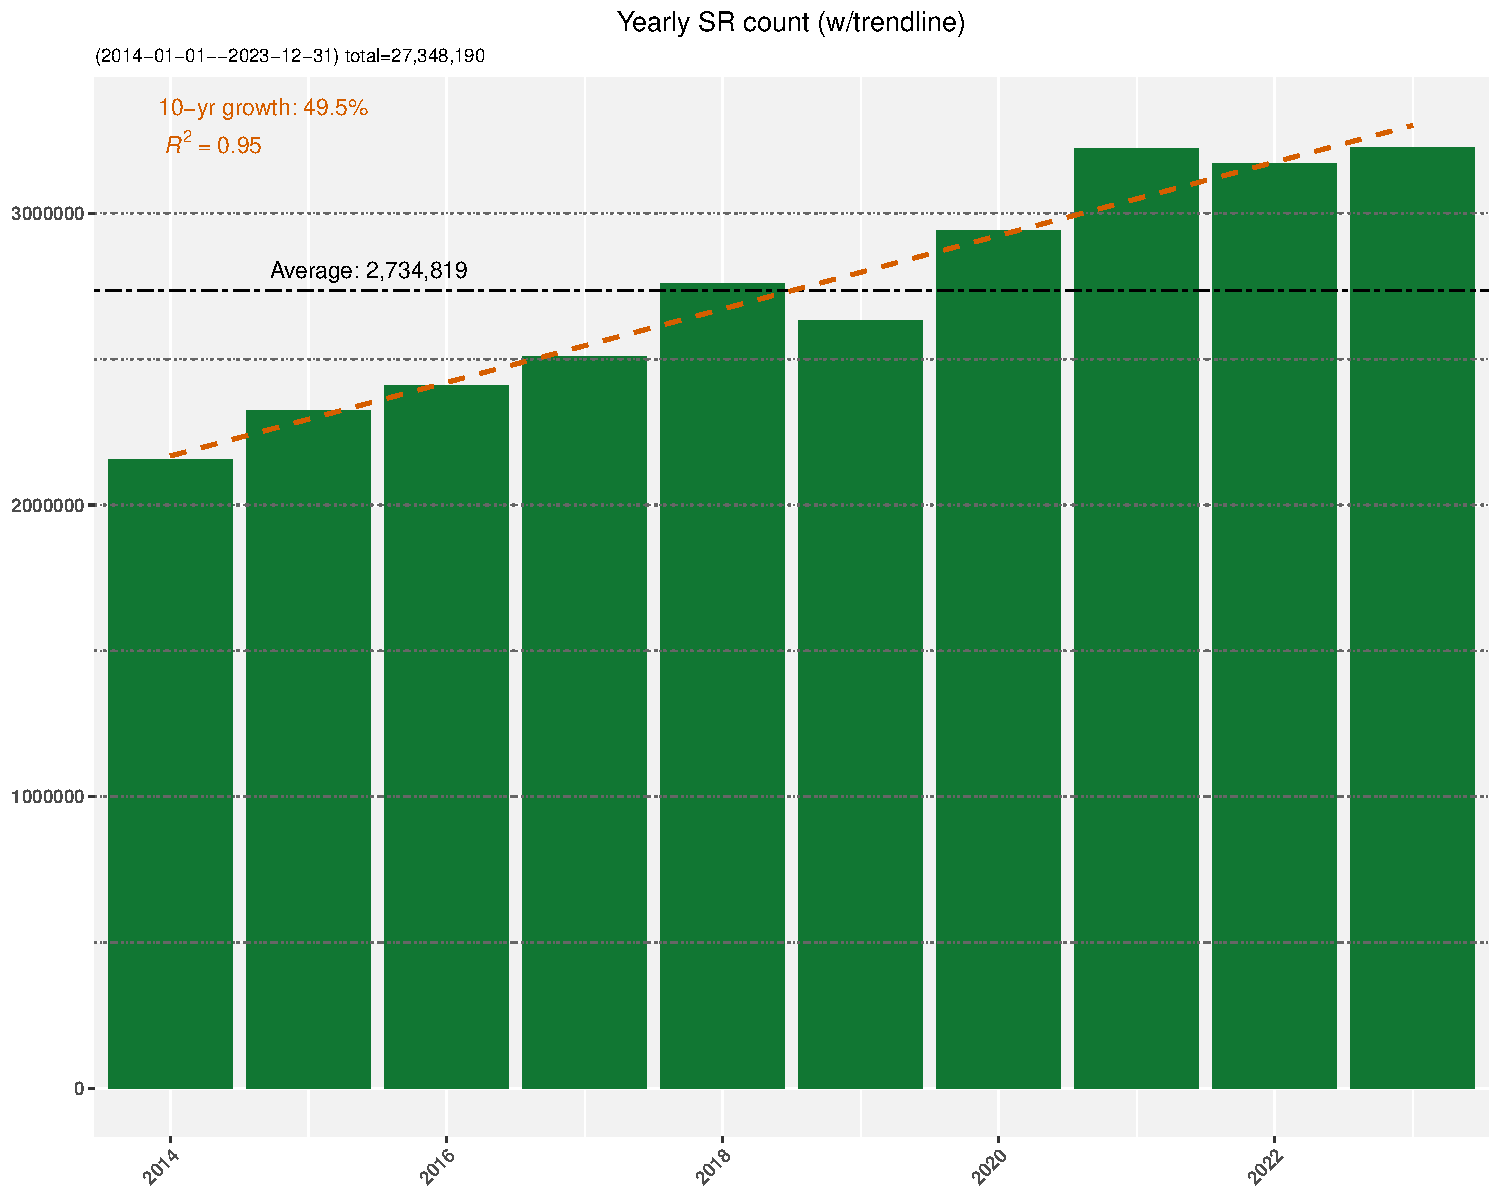
\includegraphics[width=0.8\textwidth]{10-year-trend_yearly.pdf}
 	\caption{10-year (2014-2023) Monthly SR Counts}
  	\label{fig:10-yr-monthly}
\end{figure}


Identifying the responsible agency is essential 
for troubleshooting discrepancies. This identification also assists in 
determining whether an issue is specific to an Agency or indicative 
of a broader, systemic problem. Six agencies account for 90\% of 
the complaints: New York Police Department (NYPD), 
Housing Preservation and Development (HPD),
New York City Department of Sanitation (DSNY), Department of
Transportation (DOT), Department of Environmental Protection (DEP),
and Department of Parks and Recreation (DPR).

\begin{figure}[tbp]
	\centering
	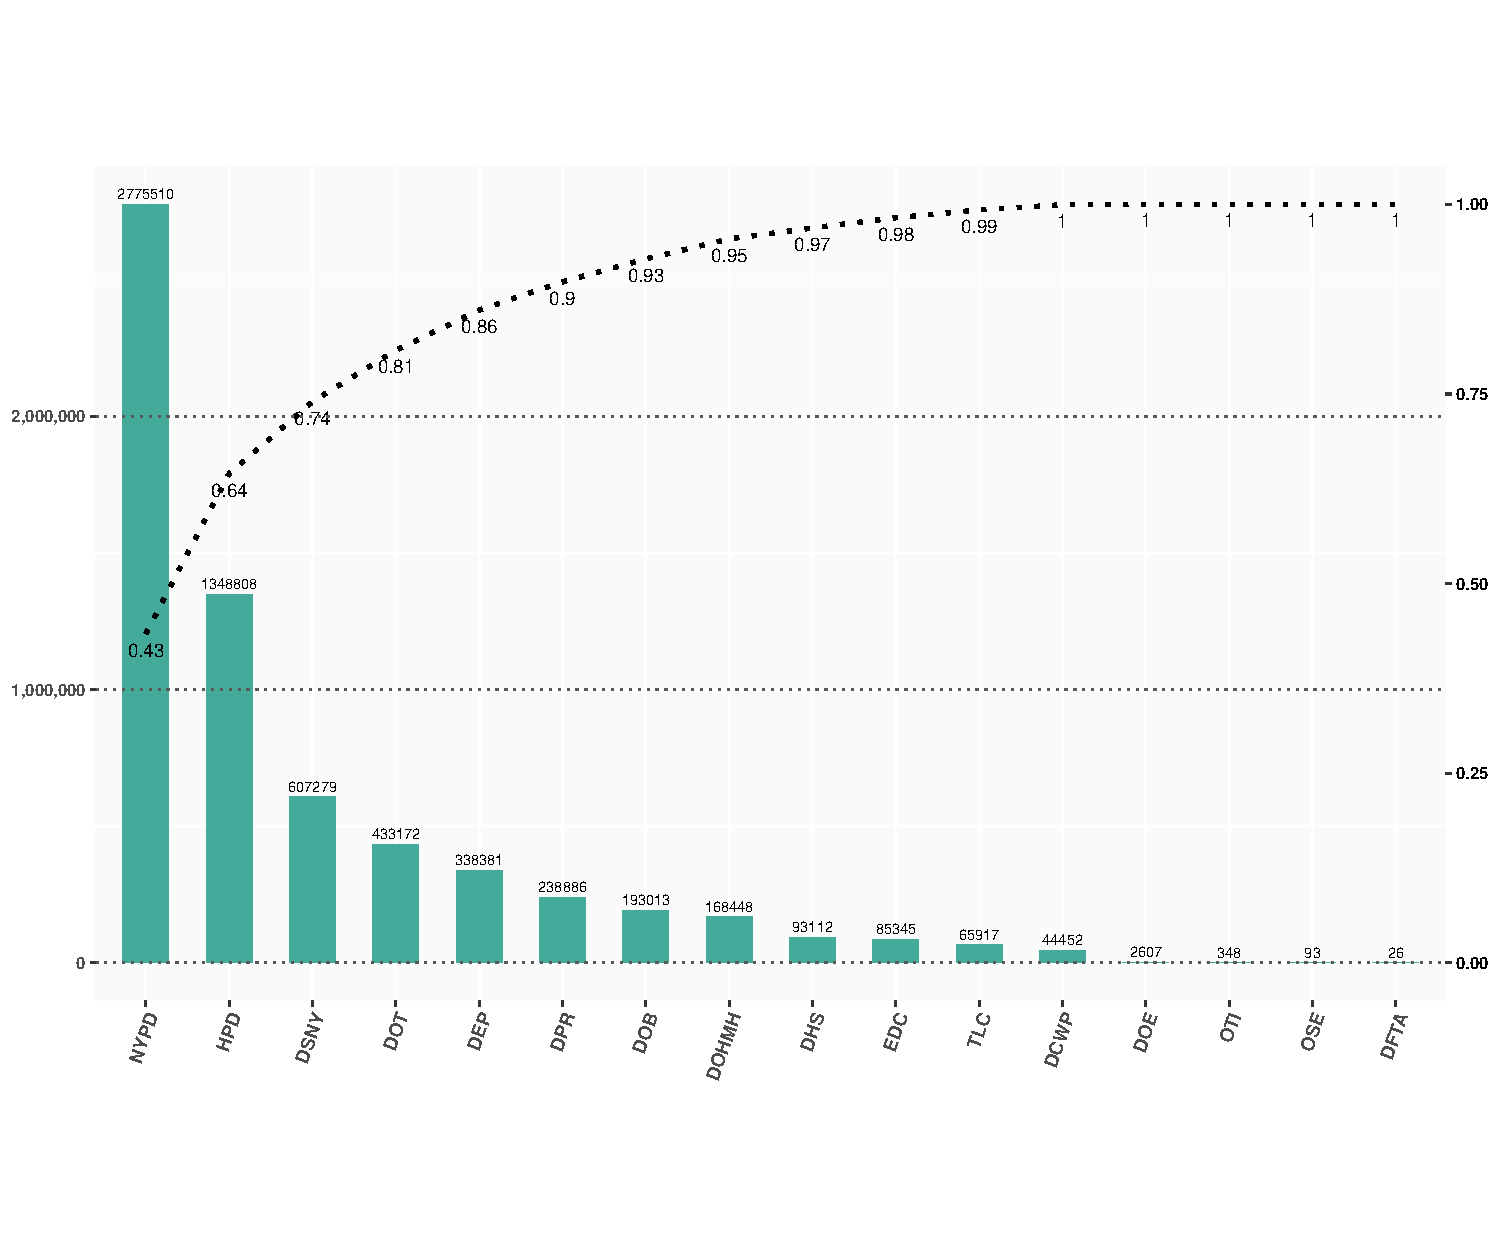
\includegraphics[width=0.8\textwidth]{SRs_by_Agency.pdf}
  	\caption{SR counts by Agency with Cumulative Percentage}
	\label{fig:SRcountbyAgency}
\end{figure}


\begin{comment}
\begin{table}[tbp]
  \centering
  \caption{Noise-related complaints\_type(s) by count with Agency}
  \label{tab:noisecomplaints}
  \begin{tabular}{@{}lS[table-format=7.0,round-mode=places,
    round-precision=0]S[table-format=2.2,round-mode=places,
    round-precision=2]l@{}} % 'l' for left-aligned, 'S' for siunitx number alignment
    \toprule
    \textbf{complaint\_type} & \textbf{Count} & \textbf{Percentage} & \textbf{Agency} \\ 
    \midrule
    Noise - Residential        & 675502 & 10.56 & NYPD  \\ 
    Noise - Street/Sidewalk    & 300507 &  4.70 & NYPD  \\ 
    Noise - Commercial         & 128892 &  2.02 & NYPD  \\ 
    Noise - Vehicle            & 115956 &  1.81 & NYPD  \\ 
    Noise                      & 100413 &  1.57 & DEP   \\ 
    Noise - Helicopter         &  85345 &  1.33 & EDC   \\ 
    Noise - Park               &  16620 &  0.26 & NYPD  \\ 
    Noise - House of Worship &   2757 &  0.04 & NYPD  \\ 
    \bottomrule
  \end{tabular}
\end{table}
\end{comment}


Figure~\ref{fig:SR_complaints} shows that the top 20 complaint 
types account for 70\% of the total 220 different types. Notably, 
these top complaints include several variations of noise-related 
issues, which collectively represent 22\% of all complaints, the 
most frequently occurring type of complaint.

\begin{figure}[tbp]
 \centering
  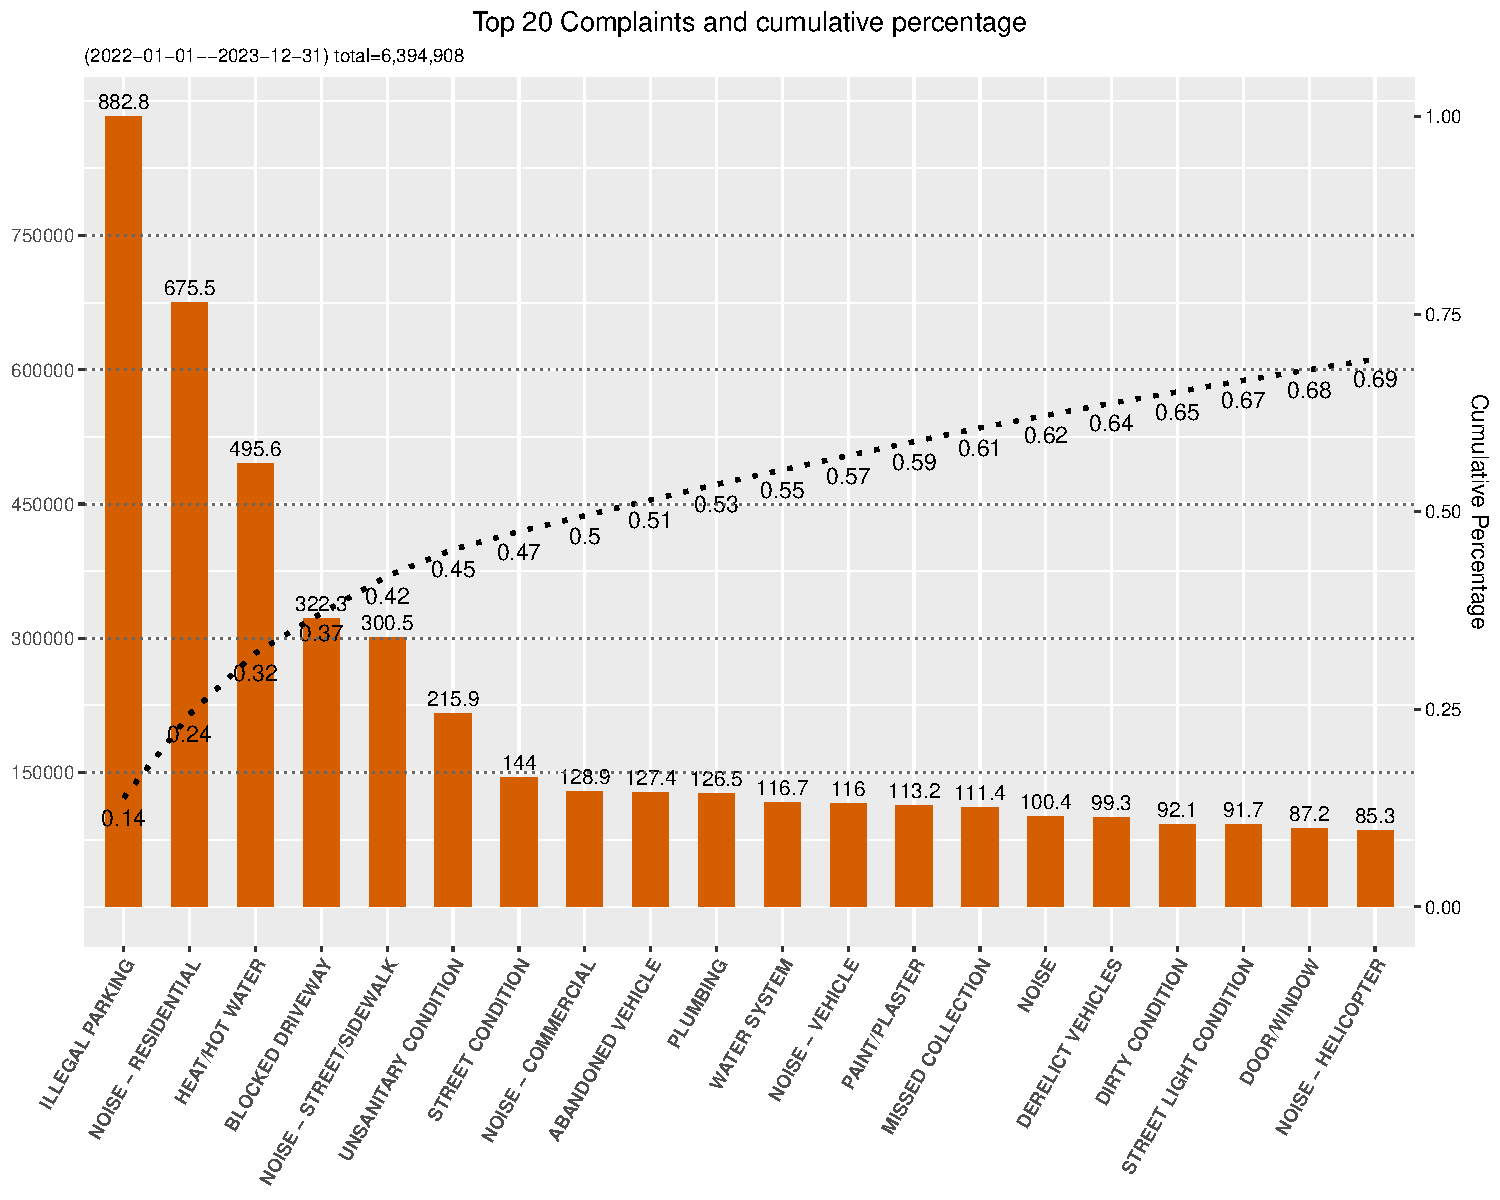
\includegraphics[width=0.8\textwidth]{SR_by_Complaint_Type.pdf} 
  \caption{Top 20 complaint type(s) and Cumulative Percentage} 
  \label{fig:SR_complaints}
\end{figure}


\section{Data Cleansing Issues} 
\label{sec:issues}

Data cleansing refers to the process of identifying and rectifying
errors, inconsistencies, and inaccuracies within datasets to ensure
they are of high quality and reliable for analysis
\citep{maletic2005data, hosseinzadeh2023data}. The process
typically involves removing duplicate records, handling missing or
incomplete data, correcting mislabeled or inaccurate entries, and
standardizing data formats. In the context of open data, cleansing is
especially important as open datasets often come from diverse,
uncoordinated sources, leading to variations in data quality,
completeness, and consistency. Without proper cleansing, the utility
of open data can be severely limited, affecting its reliability for
research, policy-making, and innovation. The main purpose of cleansing
open data is to ensure that it is accurate, consistent, and usable
across multiple platforms and by various stakeholders. This improves
the trustworthiness of the data and enables better decision-making,
more accurate analysis, and the integration of data into machine
learning models or other systems.


% What is data cleansing?  Wikipedia 
% \href{https://en.wikipedia.org/wiki/Data_cleansing}{Data Cleansing} 
% offers this definition. 

% \begin{quote}\textit{Data cleansing or data cleaning is the process of detecting and 
% correcting (or removing) corrupt or inaccurate records from a record set, 
% table, or database and refers to identifying incomplete, incorrect, 
% inaccurate or irrelevant parts of the data and then replacing, 
% modifying, or deleting the dirty or coarse data.}
% \end{quote}

Many quality criteria are utilized in order to process high-quality 
data, including:
\begin{comment}
\begin{itemize}
	\item Data validation - this effort can span a number of criteria
	
	\begin{itemize}
		\item Mandatory fields: Certain data fields cannot be empty.
		
		\item Data-types: Certain fields must be of the correct type, e.g. numeric, 
		character, date, 5 numeric digits, etc. Typically these are specified 
		in a Data Dictionary.
		
		\item Domain compliance:  Many data fields must adhere to a specific 
		domain of values, e.g. statuses, state names, zip codes, gender.
		 
	\end{itemize}   
	\item Structural errors to include naming conventions, 
	 fields not in the Data Dictionary, or inconsistent data entry. For example 
	 intermixing blanks, spaces, NA, N/A, and \textless{}NA\textgreater{} 
	 all to indicate the absence of data.
	 
	\item Redundant, unnecessary, or irrelevant fields
	
	\item Logical inconsistencies such as related fields that violate the 
	nature of that relationship, e.g. a ``due date'' that is before the ``created date''
	
	\item Accuracy versus precision
\end{itemize}
\end{comment}

This purpose of this analysis effort is to identify the presence of 
errors; not necessarily to correct them. A correction effort should
be undertaken only after an investigation as to the why and how 
such errors came about, and a discussion as to whether or not it 
even is an \textit{error}. 


\subsection{Structural Issues}
\label{sec:structural}
Structural issues refers to how data is organized, formatted, 
or presented within a dataset. Structural issues can make 
it difficult to analyze the data effectively. Here are some 
characteristics of the 311 SR data set:

\begin{itemize}
	\item There are 47 columns of data for each row, exportable as a CSV file.
	
	\item There are four date fields (created, closed, updated, due).
	
	\item There are three borough fields; two of which appear to be duplicates.
	
	\item Two zip code fields, but not duplicates
	
	\item Seven street fields; two pair of which appear to be duplicates
	
	\item Two Police Precinct fields; not duplicates
	
	\item In addition to the incident\_address, there are five additional location fields: 
	lat/long, street\_name, landmark, NY State plane, and Block \#
	
	\item One free-form text field, resolution\_description, which 
	supports 934 characters of input, including commas and special characters
\end{itemize}

The 311 SR \href{https://data.cityofnewyork.us/api/views/erm2-nwe9/files/b372b884-f86a-453b-ba16-1fe06ce9d212?download=true&filename=311_ServiceRequest_2010-Present_DataDictionary_Updated_2023.xlsx}{Data Dictionary}
 identifies 41 data columns (fields) and related information 
 for each column. However, when downloaded the data reveals 
 six additional fields that are not included in the Data Dictionary. 
(Note that these fields do show up on the portal Column Manager widget
 as ``@computed\_region\_xxxx\_xxxx''.) To some extent one can infer 
 what the these @computed\_fields are and how they are determined, but
 not with certainty. Most importantly is the question, can these fields be reliably 
 used for analytical purposes?  These six ``computed'' fields are:

\begin{itemize}
	\item zip\_codes
	
	\item community\_districts
	
	\item borough\_boundaries
	
	\item city\_council\_districts
	
	\item police\_precincts
	
	\item police\_precinct 
\end{itemize}	

		
\subsection{Blank \& N/A data}
\label{sec:blanks}
Understanding the absence of data by field is important 
when undertaking analysis. For example, if you wanted to 
determine if SRs were closed before or after their due\_date, 
you would be challenged as 99.6\% of the due\_date field is 
blank. When counting fields for blank or N/A values, they appear 
to divide into three groups: \textbf{Mostly Empty}, \textbf{Partially Empty}, 
and \textbf{Few/None Empty}. 

The Mostly Empty category ranges from 93-99.9\% blank 
and includes such fields as taxi\_company due\_date, pickup\_location, and 
landmark. The Partially Empty includes such fields as location\_type, borough, 
and cross\_street. And the Few/None Empty includes created\_date, 
complaint\_type, agency, and status. In some cases it may make 
sense to inquiry as to why some fields are frequently blank. Here is a graphic 
depiction of total empty (blank \& N/As) for each fields illustrating
the grouping into the Most, Partial, and Few categories. 


\begin{figure}[tbp]
	\centering
  	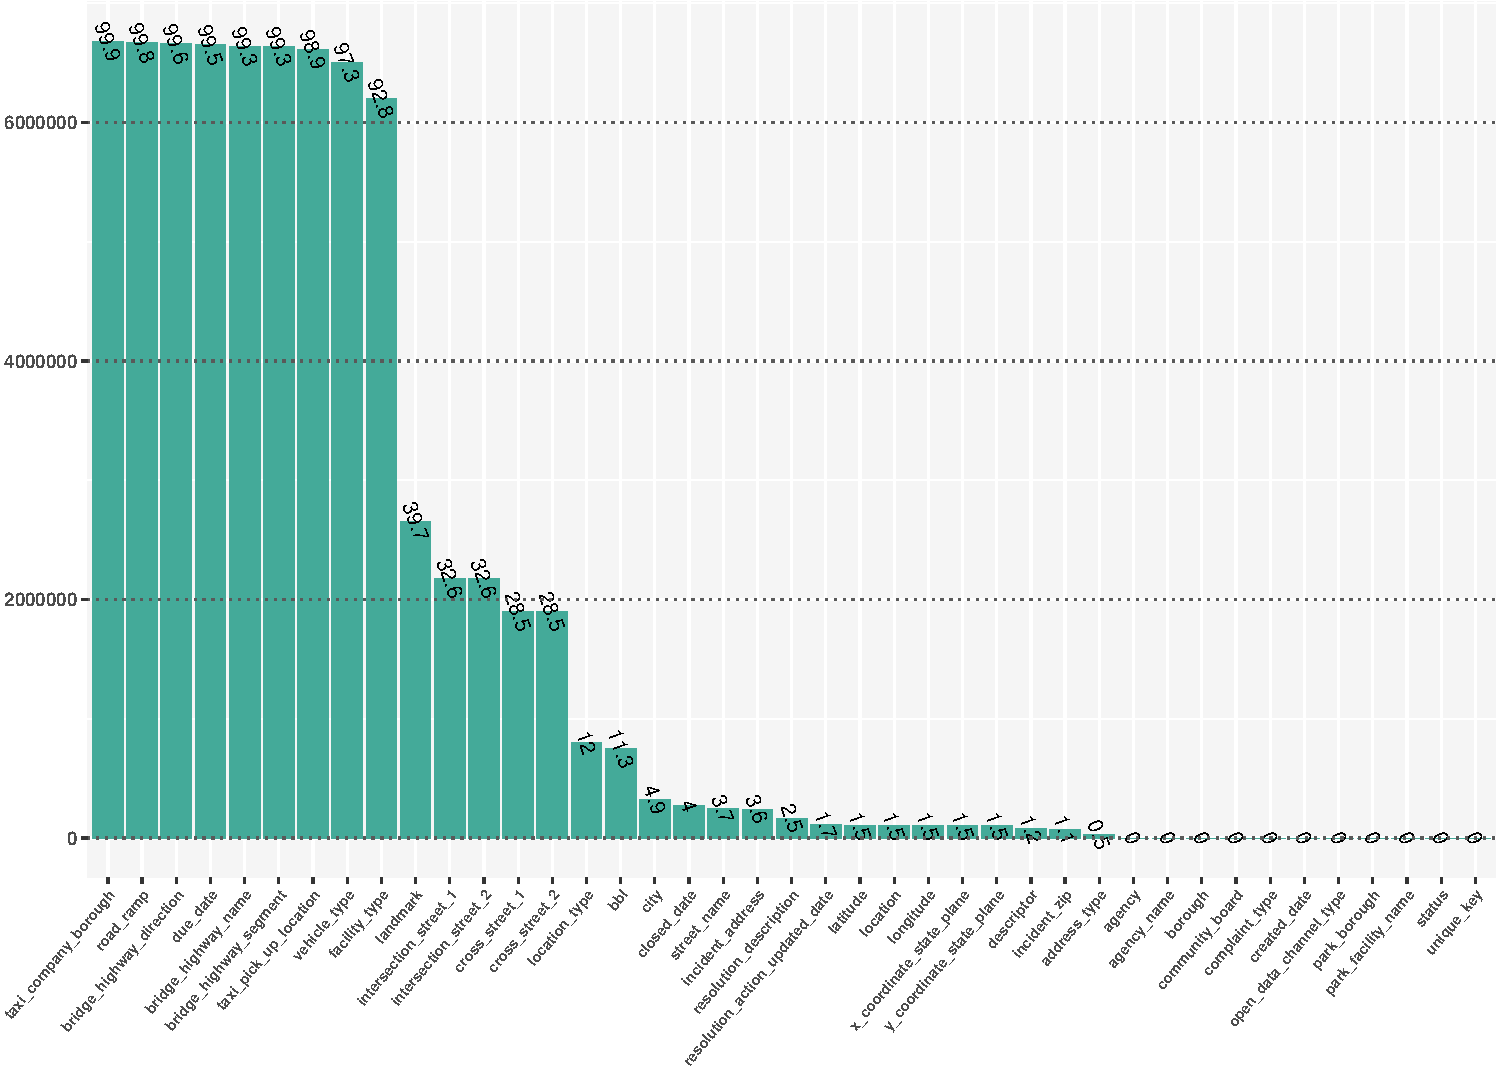
\includegraphics[width=\textwidth]{BlankFields.pdf}
	\caption{Number and Percentage of Empty/Blank Entries}
	\label{fig:blank_fields}
\end{figure}

\begin{comment}
 \subsection{Validating Data for Acceptable Values}
 \label{sec:domain}
Any analytic effort needs to be aware of fields which 
contain invalid values. Typically such fields would be
identified and removed from the analysis. Here are the results
of selected field validation.

\begin{itemize}
	\item Latitude and Longitude fields fall within the geographic 
	boundaries of New York City. 
	
	\item The unique\_key field was in-fact unique.
	
	\item Unfortunately, very few domains of acceptable 
	values are specified in the Data Dictionary. The below 
	fields were tested as complying with their domain as 
	determined by public usage and historical datasets:
	
	\begin{itemize}
		\item address\_type
		\item status
		\item borough, borough\_boundaries, \& park\_borough 
		\item data\_channel
		\item vehicle\_type
		\item city\_council\_district
	\end{itemize}	
	
\end{itemize}
\end{comment}

\label{sec:zipcodesissues}
 \textbf{Issues with Zip Codes:} Some fields proved to be problematic 
 as to their compliance with a domain of legal values. For example, all zip codes 
 (two fields: zip\_codes and incident\_zip) should be valid as defined 
 by the USPS database containing all 37,946 valid zip codes. However,
 the computed field zip\_codes proved problematic with over 
58\% (3.6 million) of the field entries being invalid. And while the more accurate 
incident\_zip field has only .07\% invalid entries, it still contains
4163 such errors; not insignificant. The breakdown of the invalid 
entries in the zip\_code, sorted by Agency shows that the 
distribution by percentage mirrors the overall breakdown of 
SRs by Agency, potentially indicating a systemic problem.
	

\label{sec:case-study-zip-codes}
\textbf{Case Study: Noise Complaints by Zip Code.}  Scenario: The NYC 
Office of Nightlife (ONL) wants to know ``What are the top 10 
zip codes for Noise Complaints over the last two years?'' ONL wants
to assess the impact of recent efforts promoting a vibrant nightlife 
in NYC while seeking to ease strained relations between bar 
and club owners. Let's assume that this analysis 
uses the zip\_codes field, one of the computed fields known to 
have validity problems. We then repeat the analysis with the more 
accurate incident\_zip field. Finally, we subject these two analysis effort 
to validation against the USPS zip code database.


\begin{table}[tbp]
    \centering
    \caption{Comparison of Top Ten Zip Codes Lists}
	    \begin{tabular}{@{}lS[table-format=6.0,round-mode=places,
	    round-precision=0]c@{\hskip 0.5cm}@{}lS[table-format=6.0,
	    round-mode=places,round-precision=0]c@{}}
		\toprule
	 	\multicolumn{3}{c}{\textbf{zip\_codes}} & \multicolumn{3}{c}{\textbf{incident\_zip}} \\
	      \cmidrule(r){1-3} \cmidrule(l){4-6}
	      \textbf{Zip Code} & \textbf{Count} & \textbf{Valid?} 
	      & \textbf{Zip Code} & \textbf{Count} & \textbf{Valid?} \\
	      \midrule
	        11275 & 104556 & FALSE & 10466 & 104562 & TRUE \\
	        12420 & 27503 & TRUE & 10023 & 27972 & TRUE \\
	        12428 & 26564 & TRUE & 10031 & 25548 & TRUE \\
	        10935 & 25508 & FALSE & 10457 & 25066 & TRUE \\
	        10934 & 23448 & FALSE & 10453 & 24752 & TRUE \\
	        10931 & 22381 & TRUE & 10456 & 24751 & TRUE \\
	        10930 & 22121 & TRUE & 10452 & 22527 & TRUE \\
	        17613 & 21963 & FALSE & 10025 & 21705 & TRUE \\
	        10936 & 21707 & FALSE & 10458 & 21689 & TRUE \\
	        11606 & 21435 & FALSE & 10032 & 20622 & TRUE \\
	      \bottomrule
	    	\end{tabular}
 	\label{tab:zipcodes}
\end{table}


As indicated, six out of ten zip\_codes are invalid, which corresponds closely 
with what is observed in the overall dataset (58\% invalid). Whereas 
the incident\_zip field is completely valid, in-line with the 
overall incident\_zip validation percentage of 99\%.


\label{sec:police-precincts}
\textbf{Issues with Police Precincts:} A curious case exists when 
examining two (nearly) identical fields: police\_precincts and 
police\_precinct. Both of those fields are among the computed fields 
previously mentioned. Using 
\href{https://www.nyc.gov/site/nypd/bureaus/patrol/precincts-landing.page}
{NYPD Precinct listings} it is possible to determine the valid 
police precincts. What we find is that both police\_precinct 
and police\_precincts  have about 35\% invalid entries. Unfortunately, 
it's not the same invalid entries. The police\_precincts field, 
has 2,171,864 invalid entries (35\%). Similarly the 
police\_precinct field has 2,171,778 invalid entries 
(also 35\%), but not the same invalid entries. 


\label{sec:communityboards}
\textbf{Issues with Community Boards:} Community Boards are the most 
local, grassroots form of City government; a vital connection 
between communities, elected officials, and City agencies. Community 
Boards often service as a measure of the equity of City services 
throughout the five boroughs. In the 2022-2023 dataset there 
are 27,276 invalid community\_board entries representing 0.43\% 
of non-blank data. The distribution of invalid Community Boards 
by Agency is not consistent with the overall SR Agency distribution,
indicating that there are likely issues at key Agencies, in 
this case Taxi \& Limo Commission (TLC), DPR, etc. 


\label{sec:communitydistrict}
\textbf{Issues with Community Districts:} Another of the computed fields 
is community\_districts. Community Districts 
are the geographic boundaries for the Community Boards, but differ as they
are used by the Department of City Planning (DCP) for environmental, 
socio-economic, and demographic purposes. It is a geographical 
division rather than a City government division. Due to how the 
community\_district data is formatted, it is not possible to 
establish validity. However, we can determine that the dataset 
contains 72 unique entries, while there are only 59 
valid Community Districts. 
	

\label{sec:negativeduration}
\textbf{Issues with created\_date and closed\_date - Negative Durations:} For 
the created\_date and closed\_date fields, one might 
expect that these two fields are automatically populated by the 
SR application software; associated with perhaps setting an SR status 
to ``new'' or ``closed''. Unfortunately, that does not appear 
to be the case as there are several anomalies with the various date 
fields:


	
\begin{itemize}
	\item SRs with a closed\_date that occurs before the created\_date.

 	\item created\_date(s) and closed\_date(s) in the far, far distant past.

 	\item created\_date(s) and closed\_date(s) that match to the second.

	\item A large number of SRs closed and/or created exactly at midnight 
	or exactly at noon, to the second.
\end{itemize}
	
	
Citizens, NYC Government Officials, and NYC Agencies especially use 
the closed and created dates as a measure of the ``duration'' of the SR 
and hence Agency responsiveness of a service. Duration, while 
not directly present in the dataset, is easily 
computed by (closed\_date - created\_date).
	
Closed-before-Created: There are 12,251 SRs that are closed before they 
were created, thereby generating a nonsensical ``negative duration''. 
While this is a small percentage overall (0.2\%) these errors can 
have significant impact on response time analysis. Here is a sample:


\begin{table}[tbp]
    \centering
    \caption{Largest Negative Duration errors (days)}
	    \begin{tabular}{l l l r l}
	        \toprule
	        \multicolumn{5}{c}{\textbf{Largest errors (days) excluding 
	        extreme negative values}} \\
	        \midrule
	        \textbf{created\_date} & \textbf{closed\_date} & \textbf{duration} 
	        & \textbf{agency} \\
		        \midrule
		        2023-01-27 14:40:00 & 2022-01-14 14:40:00 & -378.0 & DOT \\
		        2023-01-18 10:06:00 & 2022-01-12 10:06:00 & -371.0 & DOT \\
		        2023-01-27 14:36:00 & 2022-01-22 14:35:00 & -370.0 & DOT \\
		        2023-01-11 11:10:00 & 2022-01-09 11:10:00 & -367.0 & DOT \\
		        2023-12-18 03:13:00 & 2023-01-16 13:10:00 & -335.6 & DOT \\
		        \bottomrule
	    \end{tabular}
    \label{tab:largest-errors}
\end{table}

	
As noted, the largest errors are shown ``excluding extreme negative values''. We found 
eight SRs with extremely large negative durations (\textless{} -730), all originating
with DHS and all containing an entry of ``1900-01-01'' as the closed\_date. This 
generates extremely large negative durations exceeding -44,601 
days (-122 yrs). Such a large of an anomaly can significantly skew statistical 
results, even though the number of occurrences is small. According, these 
SR rows are removed from the analysis. Excluding these extreme negative
values, an analysis shows the negative-duration issue is a DOT problem, 
where 95\% of these types of errors occur. 
	
	
This violin chart shows the broad spread of negative-duration SRs, albeit with 
the extremely large negative-duration SR removed. While there are few 
outliers, the magnitude of the negative-durations is troubling and can 
produce bizarre analytical results.


\begin{figure}[tbp]
	 \centering
 	 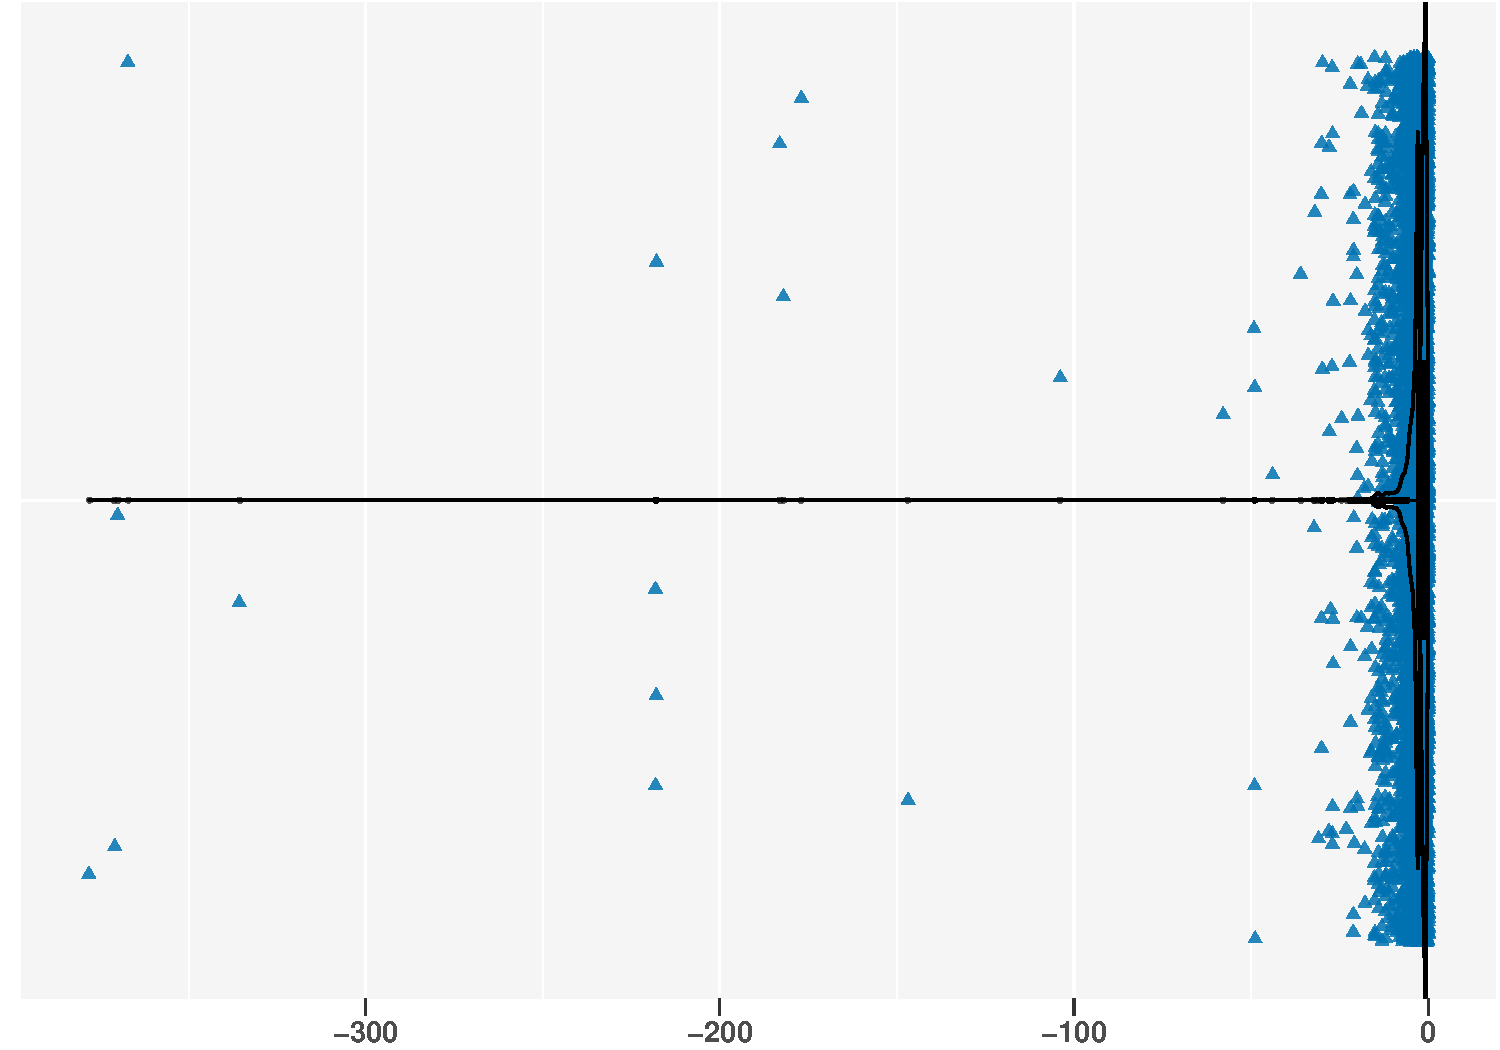
\includegraphics[width = \textwidth]{negative_duration_SR_violin.pdf}
 \caption{Distribution of Negative Durations}
 \label{fig:negative-duration-violin}
\end{figure}


\label{sec:homlessassistance}
\textbf{Case Study: Homeless Person Assistance.} Scenario: DHS wants to know ``How 
quickly have 311 SRs for ``Homeless Person Assistance'' been resolved 
over the past two years?'' This is a typical request made by 
both the public and City government; analogous to ``How quickly 
is my Agency responding to ``critical'' requests, and does 
that performance vary by Borough, Zip Code, etc. To conduct such an 
analysis, we can use the tools on the Open Data Portal. Here are the steps:
		
		
\begin{itemize}
    \item Select created\_date from 2022-2023 and filter by complaint\_type = 
    ``Homeless Person Assistance'' (this yields 55,000 SRs)
    
    \item Compute the ``duration'' (closed\_date – created\_date)
    
    \item Take an average of the ``duration'' field  which yields: \textbf{Answer:  -4.8 days}  
\end{itemize}

		
Clearly that answer is nonsensical. How did such a simple task result 
in an absurd answer? The answer lies in the computation of the ``duration'' 
field. It turns out, there are eight DHS SRs that have a closed\_date 
of ``1900-01-01''. Each of those SRs creates a negative duration of -44,602 
days (-122 years). Those eight SRs are enough to drive the 
average duration of 55,000 Homeless Assistance SRs to a negative 
value; clearly incorrect. In this case, the median is a better measure 
of central tendency. The median is  0.2 days (approx 5 hrs) which will
surely please the DHS. 

		
%\begin{figure}[tbp]
% 	 \centering
 %	 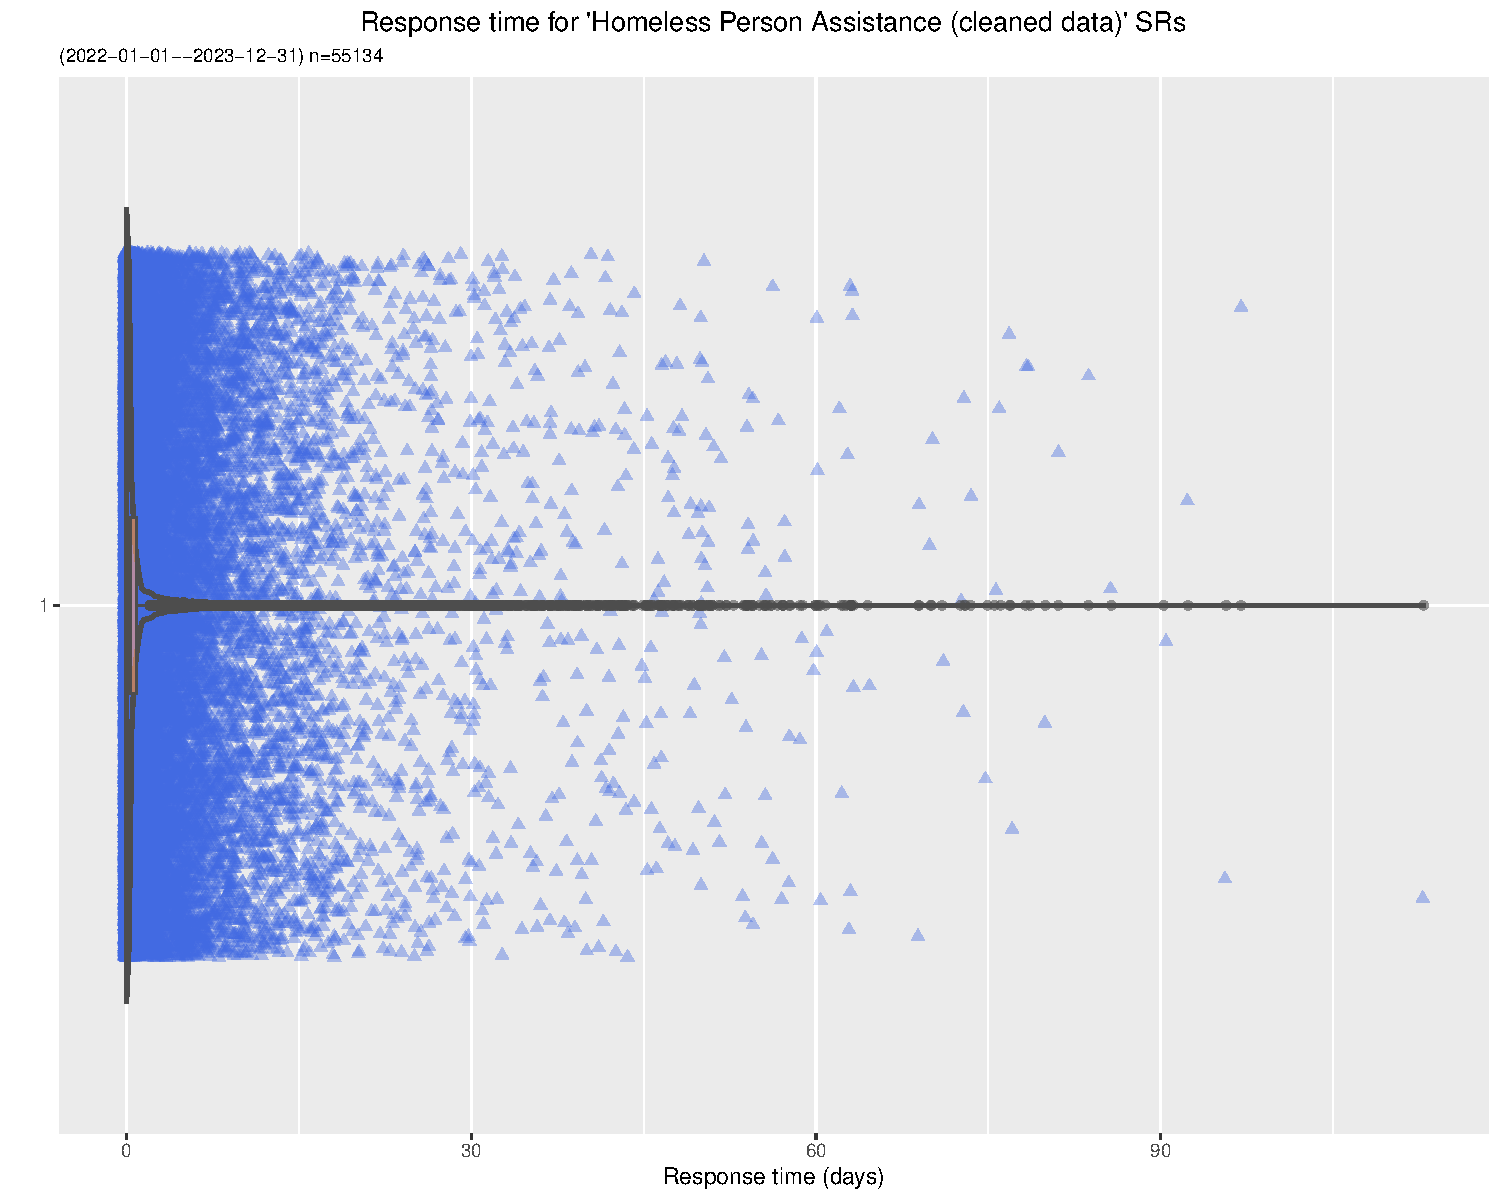
\includegraphics[width = \textwidth]{homeless_response_time_clean.pdf}
%	 \caption{Homeless Assistance SR Durations}
%	 \label{fig:homeless}
%end{figure}
	
		
\label{sec: zeroduration}		
\textbf{Issues with created\_date \& closed\_date - Zero Durations:} A more 
prevalent problem occurs when the closed\_date and created\_date 
are exactly the same -- to the second. Accordingly, this creates 
a \textbf{zero duration'}, again nonsensical. There are 191,141 
such SRs representing 3.1\% of all non-blank data. 99\% of these zero duration 
SRs occur in five Agencies:  (Dept of Mental Health \&Hygiene (DHMH), Dept 
of Transportation (DOT), Dept of Business (DOB), Dept of Sanitation 
(DSNY), and Dept of Environmental Protection (DEP). This Agency distribution
is does not mirror the overall Agency distribution of SRs, likely indicating an 
Agency-specific issue.
	
		
%\begin{figure}[tbp]
%	 \centering
%	 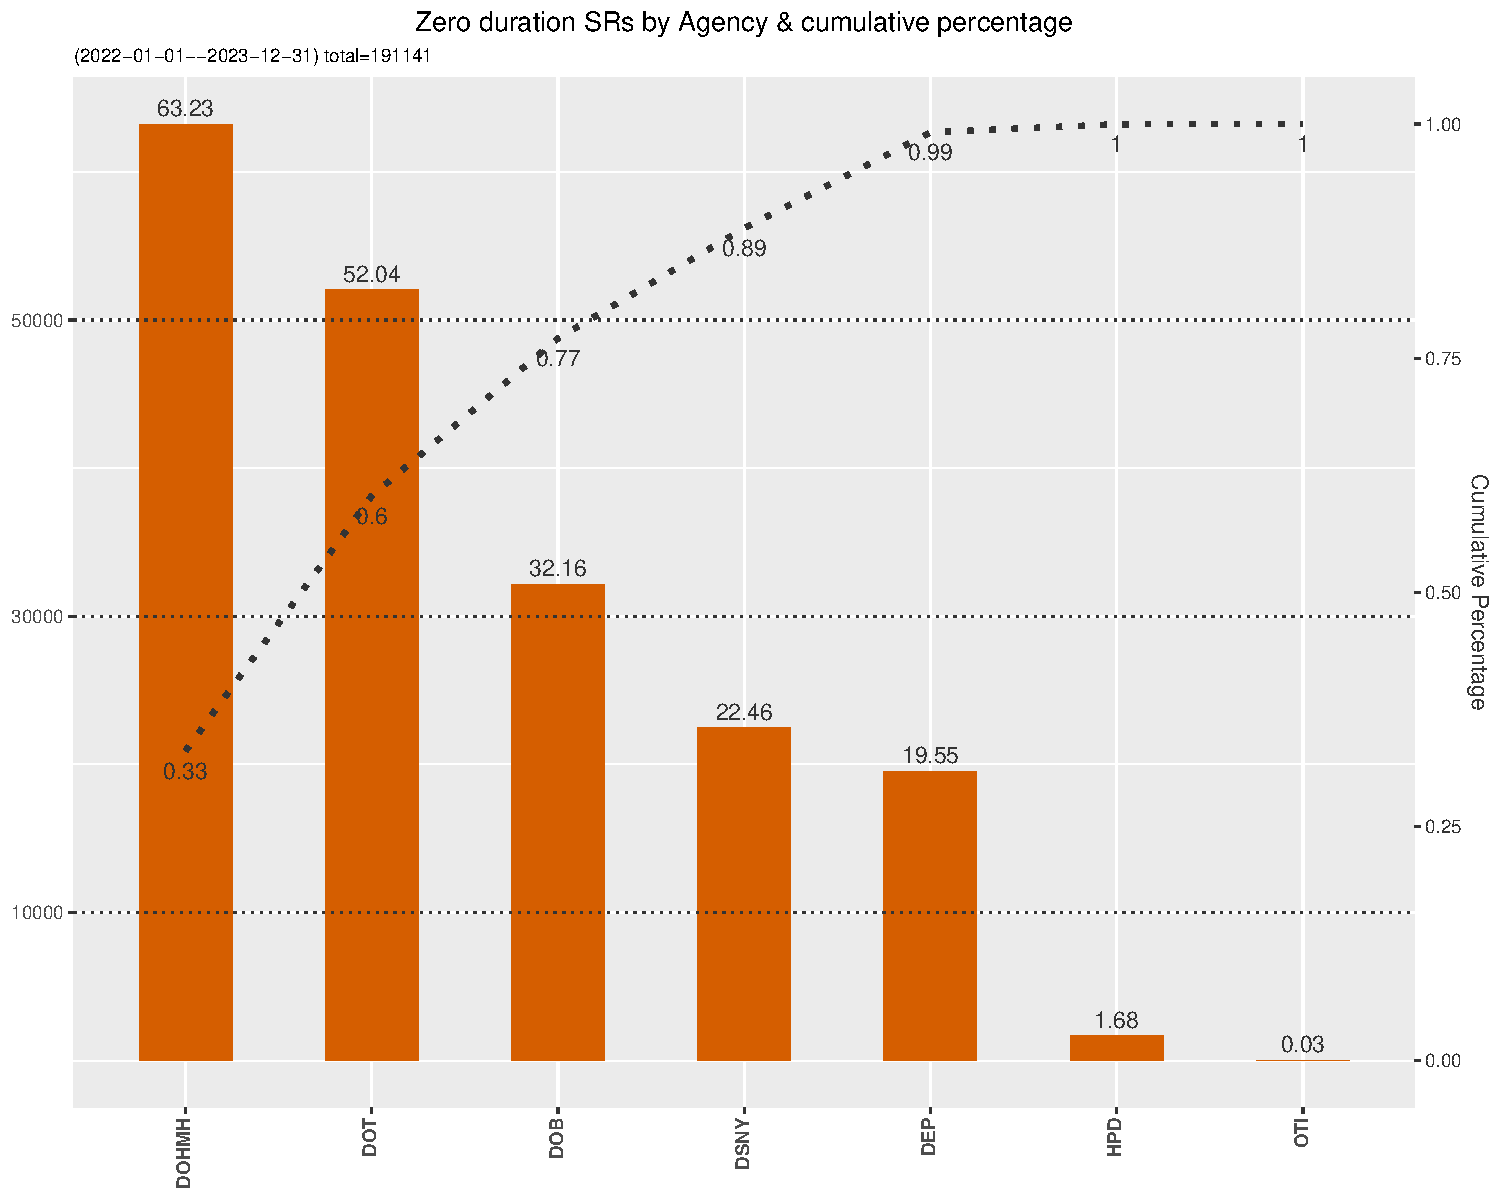
\includegraphics[width = \textwidth]{zero_duration_SR.pdf}
%	 \caption{SRs with Zero Durations by Agency}
%	 \label{fig:zero-duration}
%\end{figure}	

		
\label{sec:midnightandnoon}
\textbf{Issues with created\_date \& closed\_date(s) - Midnight \& Noon:} Another 
problem discovered with the created\_date and 
closed\_date fields - there are an unusually large number of SRs 
created or closed at exactly midnight (00:00:00) and exactly noon (12:00:00), 
to the second. Normal distribution of SR creation and closure 
largely follows the work-day clock with most  SRs created during 
day-light hours, and fewer SRs 	created at night and the early hours 
of morning. However, there are significantly greater numbers 
of SR closed exactly at midnight and noon, as well as a significant 
number of SRs created exactly at noon. Observations include:

	
\begin{itemize}
	 \item There were 99,779 SRs created exactly at noon (12:00:00)
	
	 \item There were 235,347 SRs closed exactly at midnight (00:00:00)
	 
	\item There were 105,505 SRs closed exactly at noon. 
\end{itemize}


A unique way to visualize this anomaly is to examine the busiest day 
during this 2-year period (Friday, 2023-09-29). Then aggregate 
the created\_date(s) by minute (with seconds equal to zero), providing
a minute-by-minute look at SR creation on that one day. Note the spike 
at exactly noon (12:00), well beyond the 3\textsigma line.

\begin{figure}[tbp]
	\centering
	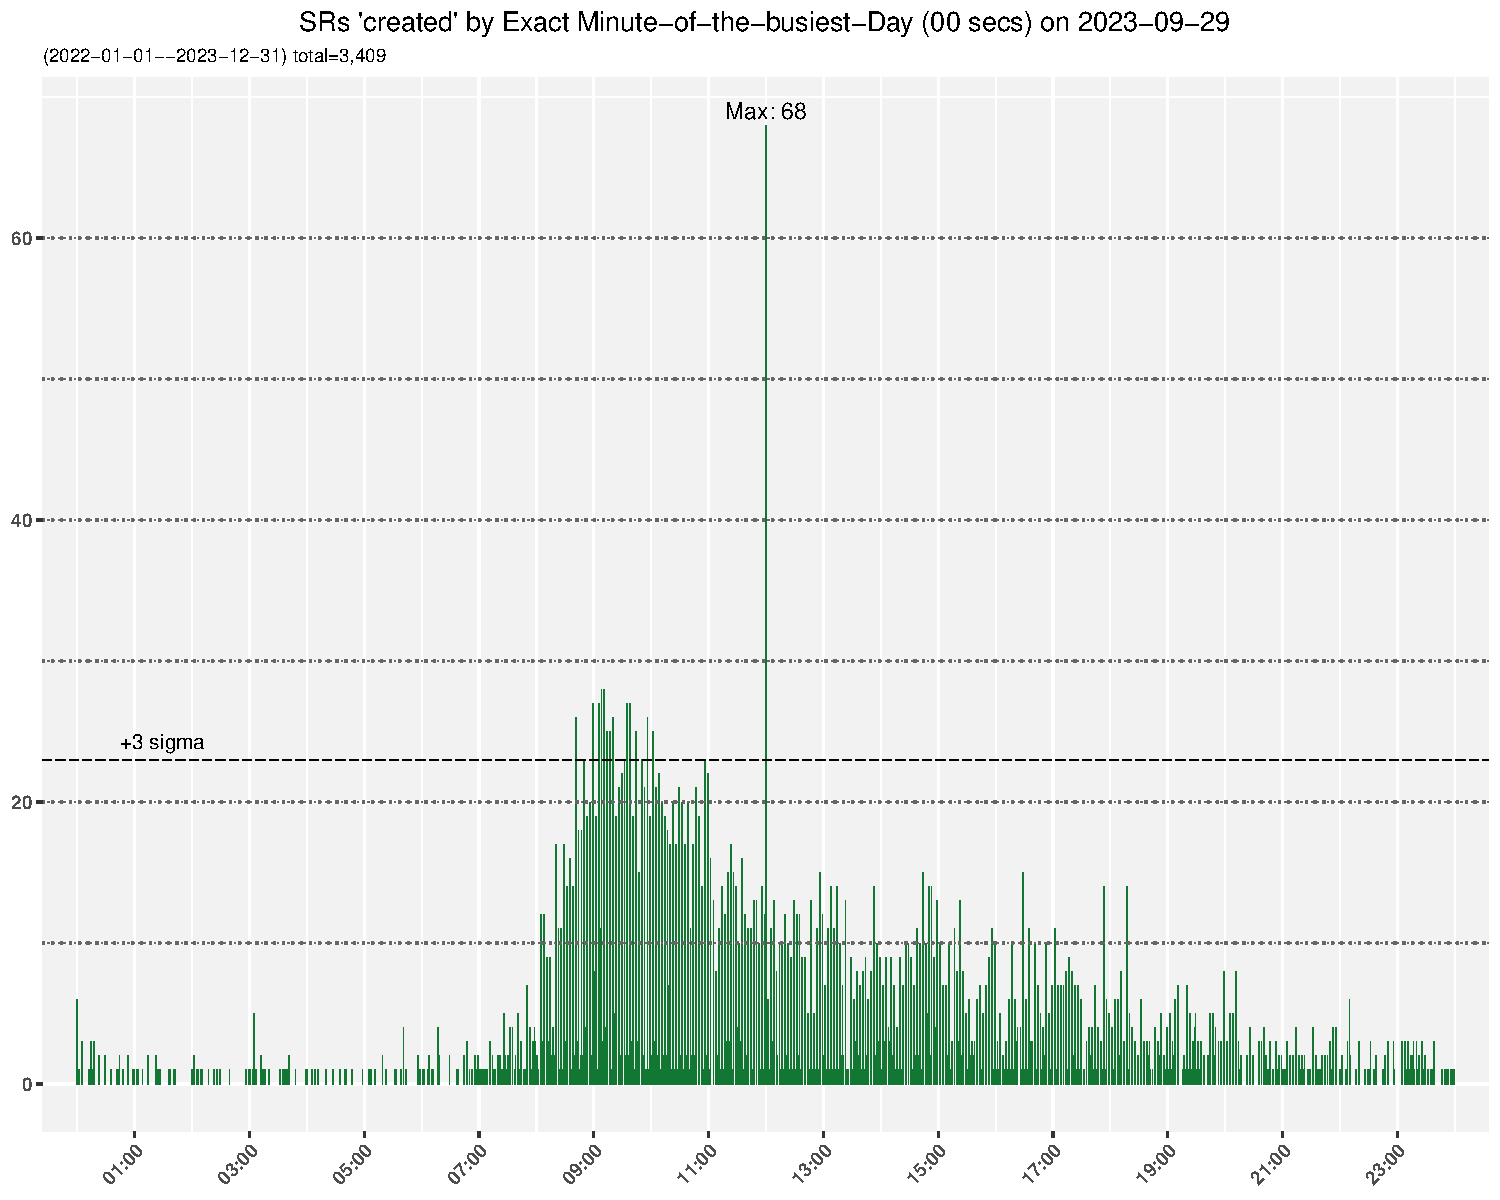
\includegraphics[width=\textwidth]
	{2-year-trend_SR_created_by_minute_of_busiest_day.pdf}
	\caption{SRs Created Minute-by-Minute on Busiest Day}
	\label{fig:busiestcreated}
\end{figure}	


Repeat the same for the \# of SRs with closed\_date(s) 
on the busiest day (Friday, 2023-09-29). Again, aggregated by 
the minute (with seconds equal to zero). Note the spikes 
at 00:00:00 and 12:00:00 respectively. 


\begin{figure}[tbp]
	\centering
	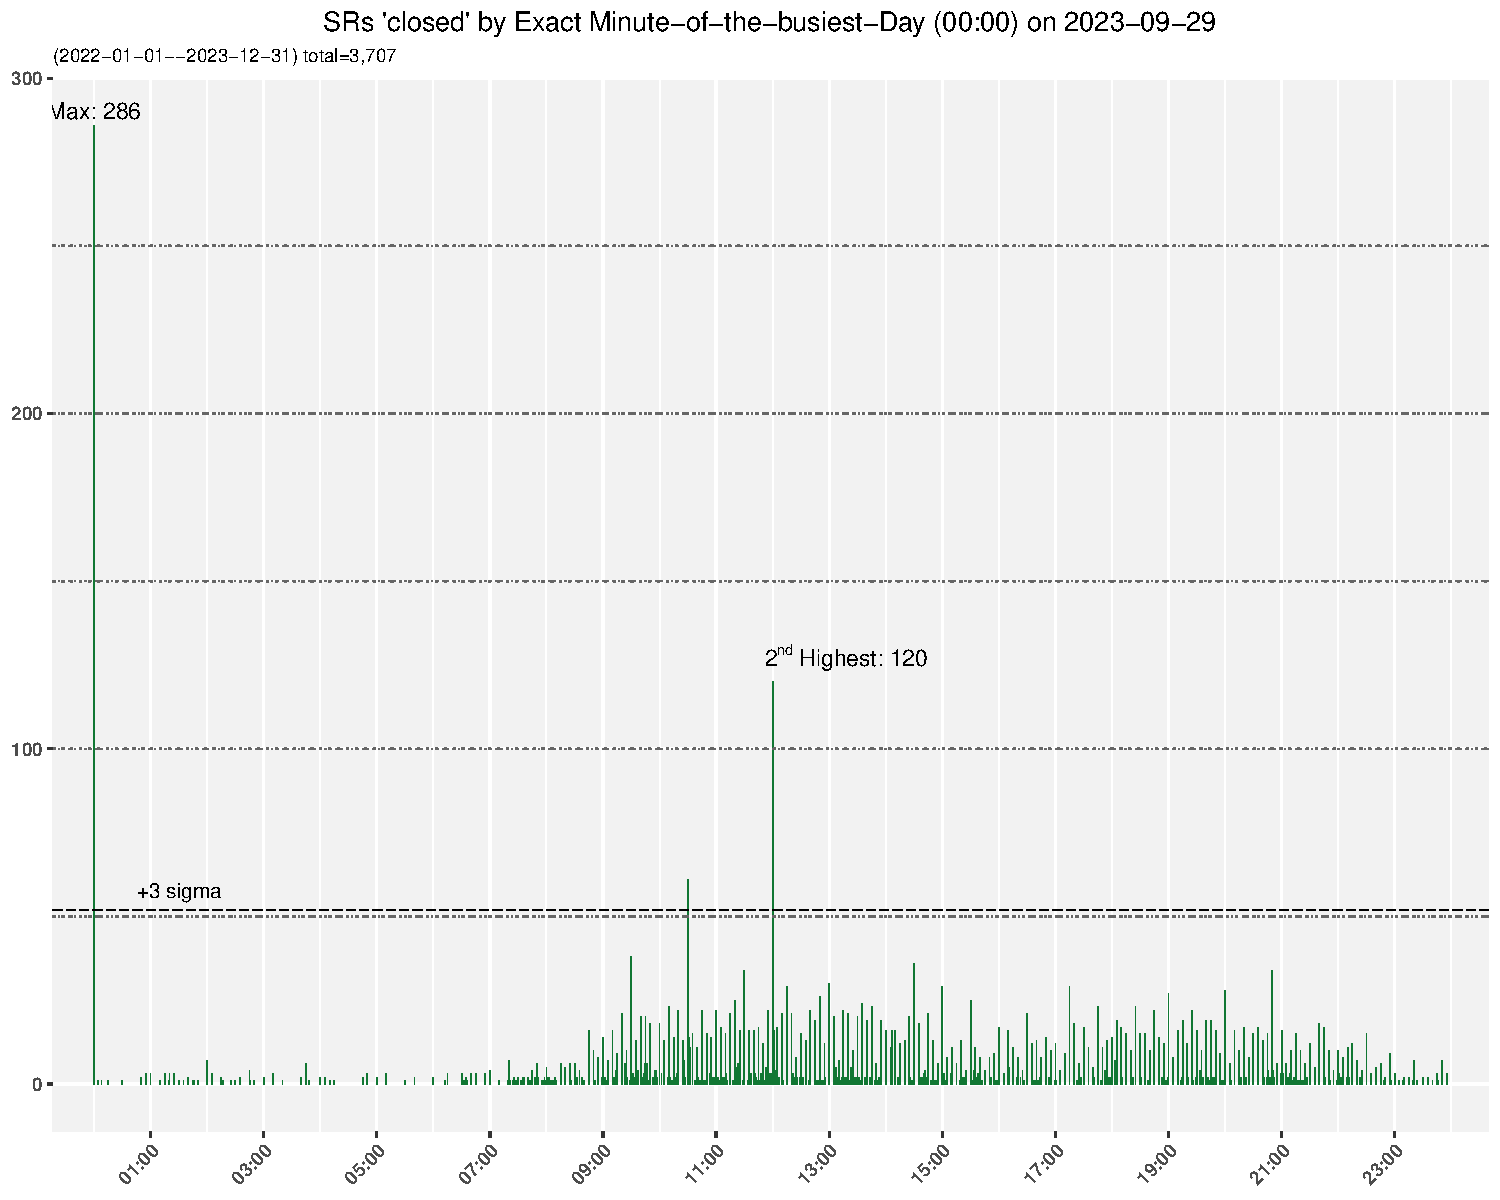
\includegraphics[width=\textwidth]{2-year-trend-SR_closed_by_minute_of_busiest_day.pdf}
	\caption{SRs Closed Minute-by-Minute on Busiest Day}
	\label{fig:busiestclosed}
\end{figure}	


These unusual patterns of created \& closed SRs at exactly the hours 
of midnight and noon likely indicates the presence of a bulk create/close 
software process that perhaps automatically ``closes'' 
(or ``creates'') a large number of SRs with a generated time-stamp of exactly 
midnight (00:00:00) or noon (12:00:00). Such behavior distorts
 the duration of these SRs by providing inaccurate dates. The 
 distribution by Agency for this anomaly indicates 
 that \textgreater90\% of these ``created\_at\_noon'' SRs come from 
 just two Agencies: DOB and DSNY.  Further investigation
 reveals that  a single Agency, DSNY, is responsible 
 for \textgreater99\% of the SRs ``closed-exactly-at-noon''. 
	

\label{sec: resolutionaction}
\textbf{Issues with resolution\_action\_update\_date:} When an 
SR is updated, the 311 software automatically 
populates the resolution\_action\_update\_date. Some of 
those  updates are happening long after the SR is 
closed. There are a total of 7460 SRs that are updated \textgreater30 days 
after the closed\_date (and \textless{}730 days to avoid infeasible 
dates such as 1900-01-01). It is not known if this is normal behavior
 or an area that requires further investigation. 
	
	
\begin{figure}[tbp]
	\centering
	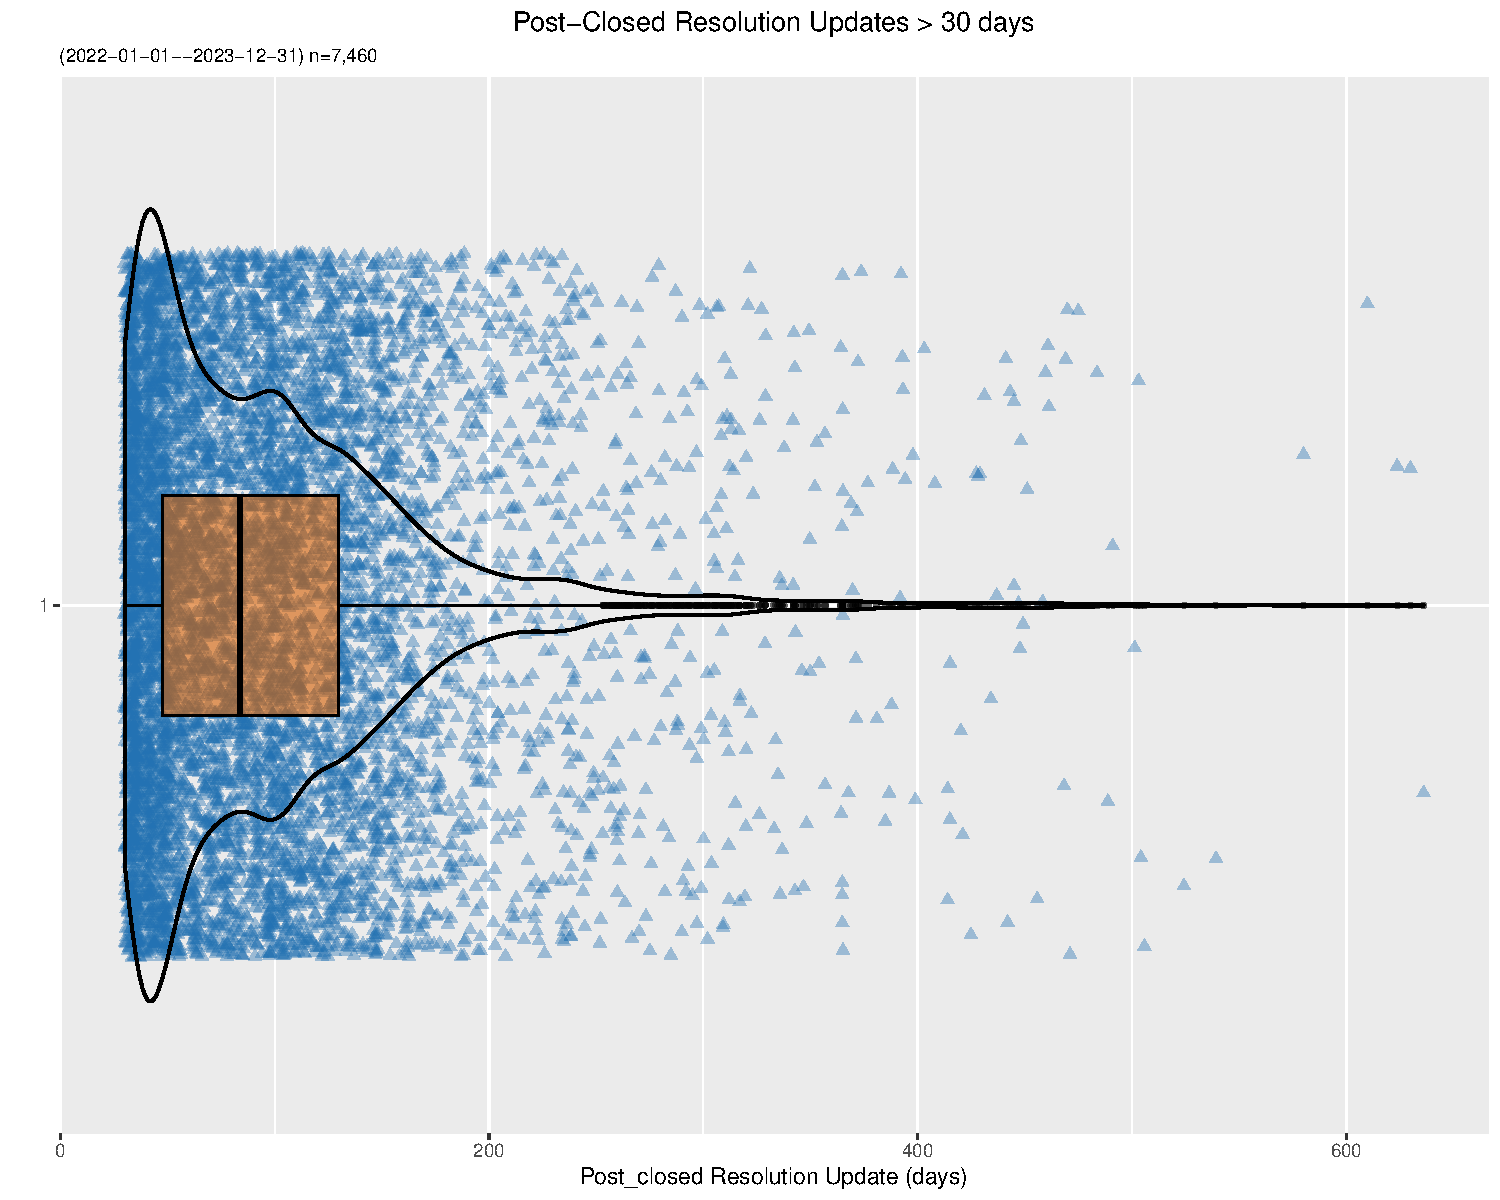
\includegraphics[width = \textwidth]{post_closed_violin_chart.pdf}
	\caption{Post-Closed resolution\_action\_update\_date(s) \textgreater30 days}
	\label{fig:resolution-violin}
\end{figure}		

	
\subsection{Accuracy and precision}
\label{sec:precision}
An question of precision vs. accuracy arises with the Latitude 
and Longitude fields. Both Latitude are expressed as 
a 14-decimal number, e.g. 40.86769186022511. Given 
that 1 degree of latitude at the equator is equal to 111.044736 
kilometers, the ``1'' at the end of that number represents 
approximately 1.1 nanometers (1/1,000,000,000 of a meter). For 
reference a DNA molecule is approximately 2nm in width. Clearly 
the representation of the Latitude and Longitude fields is a 
classic case of 14-digit precision, but limited accuracy. 


\subsection{Redundant \& Duplicate fields}
\label{sec:duplicates}
During this analysis, several redundant fields were observed which
should be examined further for possible consolidation.


\label{sec:latlong}
\textbf{latitude \& longitude and location:} The location 
field is a 100\%pure concatenation of the latitude 
and longitude fields with a comma and parenthesis 
added. Thus the  location field seems questionable as the value, 
and the data is arguably more difficult to 
extract and use than the two individual fields. Example:  


\begin{itemize}
	\item  latitude: 40.768456429488
	
	\item  longitude: -73.9575661888774
	
	\item  location: (40.768456429488, -73.95756618887745)
\end{itemize}


\label{sec:parkborough}
\textbf{borough \&  park\_borough fields:} Borough and 
park\_borough: These two fields are 100\% matches; fully redundant.


\label{sec:boroughboundaries}
\textbf{borough \& borough\_boundaries:} Borough and 
borough\_boundary fields are a 98.3\% match. This 
is an example of the the problem with two ``near-duplicate'' 
fields; which field is correct when they disagree?


\label{sec:taxicompanyborough}
\textbf{borough \& taxi\_company\_borough:} Borough and 
taxi\_company\_borough fields that despite their names, are 
nearly completely different with only a 0.05\% match, suggesting 
that these two fields are used very differently. The taxi\_company\_borough
 field is used exclusively by the TLC which governs all cars for hire. Any
 discussion of duplication with other borough-related fields 
 should include a discussion with TLC as to the usage of these similar,
 but non-matching, fields.
 

\label{sec:zipcodes}
\textbf{incident\_zip \& zip\_codes:} The zip\_code field is one 
of the six computed fields and its validity 
 was previously explored and found to be 
 lacking; 56\% of the entries are invalid. The companion 
 field, incident\_zip, had an accuracy rate of 99.93\%. Our analysis
 indicates that the computed zip\_code field should be eliminated
 or masked from the public until such time as accuracy 
 issues can be addressed. 


\label{sec:police} 
\textbf{police\_precinct \& police\_precincts:} Both the 
police\_precinct and police\_precincts are among the computed 
fields not cited in the Data Dictionary. However, their usage is easy to 
discern; they presumably represent the NYPD precinct 
corresponding to the incident address. These two 
fields are near-duplicates with 99.9\% of the entries 
matching. Since the underlying computational process 
is unknown, we are unable to determine which 
field is ``more correct'' field. However having two fields with 99.9\% 
duplicity indicates that perhaps only one police 
precinct field is necessary.


\label{sec:agencyname}
\textbf{agency \& agency\_name:} The agency and agency\_name 
fields, while not duplicates per se, have a 1:1 correspondence. The 
Agency field contains abbreviations for the City agencies, e.g. NYPD, 
DOT, HPD, DSNY, etc. The agency\_name field contains the full name 
of these organizations. It seems redundant to include both as 
the abbreviations are commonly used and well understood.


\label{sec:landmark}
\textbf{landmark \& street\_name:} The landmark field is listed 
in the Data Dictionary as ``...any noteworthy location, 
including but not limited to, parks, hospitals, airports, sports 
facilities, performance spaces, etc.'' Our analysis
found that was not the case. To be sure, many of the entries in 
the landmark field do contain landmark names, e.g.``Pennsylvania 
Station'', ``LaGuardia Airport'', etc.,  but the vast majority 
of the entries are street names, e.g. ``Fenton Avenue'', ``Steinway 
Street'', ``Broadway'', etc.. These entries are very similar to the 
street\_name field with a 62\% match, enough to be indicative 
of some level of duplicative usage. Even the non-matches 
(excluding blanks) appear to be matches except for 
minor spelling and nomenclature changes, 
e.g. ``NINTH AVE'' \& ``9 AVE''. It's worth investigating what is going on
with the usage of the landmark field.

	
\label{sec:cross-street}
\textbf{cross\_street\_1 \& intersection\_street\_1 and cross\_street\_2 
\& intersection\_street\_2: } There are two sets of street pairs provided 
in addition to the incident\_address field. These pairs are:


\begin{itemize}
	\item cross\_street\_1 \& intersection\_street\_1
	
	\item cross\_street\_2 \& intersection\_street\_2
\end{itemize}

	
These two street pairs are used to assist in identifying the address, 
as is common in New York City. These two street pairs
have 88\% duplicates where both cross\_street\_1 matches 
intersection\_street\_1 and cross\_street\_2 
matches intersection\_street\_2. We believe only one of these
street pairs are necessary, but which one? This illustrates the 
problem of two similar data fields that largely, but not exactly, match. In
this case there are 12\% that do not match; which field to trust?


\textit{(Note: Address standardization was applied to  street 
addresses using the R \textit{campfin} package. This standardization 
prevents generating a non-match between locations such as 
``240 E 69\textsuperscript{th} ST'' and ``240 E 69\textsuperscript{th} Street'' 
which are clearly the same address save for formatting 
and slight spelling differences.)}


\textbf{Near matches:} In addition to the matching values, we 
encountered a number of \textit{near-matches}; situations where the 
cross\_street and intersection\_street are nearly, but not exactly, identical. 
For example, HARMON DR and HARMON RD. To identify these near-matches 
we measured the \href{https://en.wikipedia.org/wiki/Hamming_distance}
\textit{Hamming Distance} between the two fields. The Hamming Distance is a 
measure of how many letters must be changed for the two 
fields to match. For this analysis, we chose a Hamming Distance of two (2).
 Here are some example results for near-matches for both 
 cross\_street\_1 and intersection\_street\_1. 
 (Cross\_street\_2 and intersection\_street\_2 show similar results.)


\begin{table}[tbp]
    \centering
     \caption{Near-matches for cross\_street\_1, intersection\_street\_1}
     \label{tab:x1nearmatches}
		\begin{tabular}{l l l r}
	        \toprule
	        \textbf{cross\_street\_1} & \textbf{intersection\_street\_1} 
	        & \textbf{agency} & \textbf{hamming\_distance} \\
	        \midrule
	        WEST 168 ST    & WEST 167 ST           & DOT    & 1 \\
	        105 AVE        & 107 AVE               & DOT    & 1 \\
	        145 ST         & 150 ST                & DOT    & 2 \\
	        138 ST         & 139 ST                & DOT    & 1 \\
	        19 AVE         & 20 AVE                & DOT    & 2 \\
	        76 ST          & 79 ST                 & DOT    & 1 \\
	        67 ST          & 68 ST                 & DOT    & 1 \\
	        \bottomrule
	    \end{tabular}
\end{table}

\begin{table}[tbp]
    \centering
    \caption{Summary of cross\_street\_1 and intersection\_street\_1}
    \label{tab:summary1}
	    \begin{tabular}{l r r}
	        \toprule
	        \textbf{category} & \textbf{count} & \textbf{percentage} \\
	        \midrule
	        Matching                    & 5,637,182 & 88.15     \\
	        Both blank -- Matching      & 1,624,499 & 25.4      \\
	        Non-matching                &   757,726 & 11.85     \\
	        cross\_street\_1\_blank     &   222,232 & N/A       \\
	        intersection\_street\_1\_blank &   519,348 & N/A       \\
	        Near-match                  &       128 & 0.002002  \\
	        \bottomrule
	    \end{tabular}
\end{table}


\subsection{Shrinking file size by removing duplicates}
 \label{sec:filesize}
Shrinking file size by removing duplicates: By removing duplicate 
and ``near-duplicate'' fields, it is possible to 
shrink the file size by 12.3\% which for this large dataset equates to a 
reduction of 395 Mb. A smaller file size means faster downloads, 
less storage impact, as well as simplifying data analysis efforts.  
 
 
Below is a list of duplicate and near-duplicate fields. There are 
some challenges with these proposed deletions, mostly with 
the ``near duplicate'' fields.  For example, while the park\_borough is 
a complete duplicate of the borough field, the 
borough\_boundary field is only 98.3\% duplicate. Admittedly, 
loosing 1.7\% of the data in those two fields is quite small, however
for this large dataset that small percentage still amounts 
to 110,715 non-matching occurrences. The authors  propose 
deleting the following fields from the data set.
 
 
\begin{itemize}
	\item agency\_name: Each row of data contains the agency field, 
	which is an abbreviation of the Agency's name. The agency\_name 
	abbreviations are clear, simple, and well understood.
		    
	\item park\_borough:  This field is a 100\% match with the 
	borough field, thus no data loss. 
		    
	\item location:  The location field is a straight concatenation of 
	the latitude and longitude fields, with a comma and parenthesis 
	added. The data is a 100\% duplication of the latitude 
	and longitude fields, thus no data loss.
		    
	\item police\_precinct: This field has a 99.95\% match with the 
	police\_precincts fields. We are unable to determine which field 
	is more correct, but feel that removal of one of the precinct fields 
	is prudent and would result in minimal data loss.
		   
	\item borough\_boundaries (computed field): This field is one of 
	the six computed fields. It has a 98.3\% match with the borough 
	field.
		    
	\item cross\_street\_1 \& 2 and intersection\_street\_1 \& 2: These 
	two pairs of fields each have an 88\% match. We would recommend 
	deleting the two intersection\_street (1 \& 2) fields while acknowledging 
	some loss of data in doing so.
		     
	\item zip\_codes(computed field):  This field is one of the six 
	computed fields. However, this field has error rate of 58\% and 
	as shown in the \ref{sec:case-study-zip-codes} can lead to 
	dangerous mistakes when used for analytical purposes. We 
	recommend deleting this field.
\end{itemize}
 	
 	
Additionally, it would be worth investigating if certain data fields are 
in-fact useful, as the population of these fields is very scarce. For 
example, the taxi\_company\_borough field is 99.94\% 
blank. A similar situation exists for the road\_ramp field 
(99.8\% blank), the vehicle\_type field (99.7\%blank), and 
due\_date which is 99.6\% blank. Several additional several fields
are mostly blank: bridge\_highway\_direction, bridge\_highway\_name, 
bridge\_highway\_segment, and taxi\_pick\_up\_location; all 
have \textgreater99\% blanks. Most of these latter fields 
appear to used exclusively by the TLC.  


\subsection{Data Dictionary Observations} 
\label{sec:datadictionary}
The Data Dictionary could benefit from an update. We found several 
discrepancies between the Data Dictionary and the 
actual data which can potentially lead analytic efforts astray. 

\begin{itemize}
	\item While the Open Data portal lists the data types of the 
	various fields, the Data Dictionary does not. Nor does it provide 
	information on the specifics of various fields, such 
	as constraints or the domain of legal values. For example, the 
	incident\_zip field is specified as ``text''. That is probably not the 
	best definition; perhaps	``categorical'' with a note indicating that 
	the data can contain only numeric characters and is 
	not subjected to arithmetic operations. 

	\item Many of the domain of legal values are incomplete or 
	inaccurate. For example, the Data Dictionary indicates that 
	the status field has values of \textit{assigned, canceled, closed}, 
	or \textit{pending}. However, we found additional status 
	values of: \textit{in progress, started}, and \textit{unspecified}. 
	Additionally, we found no SRs with a status of \textit{canceled}. 
	Similarly, the address\_type field is indicated to have 
	values \textit{address, blockface, intersection, latlong}, and 
	\textit{placename}. We discovered the additional values of 
	\textit{bbl} and \textit{unrecognized}. Additionally, no values of 
	\textit{latlong} were observed. Other fields (facility\_type, 
	vehicle\_type, taxi\_pick\_up\_location, road\_ramp, city) 
	suffer similar inaccuracies in their specified domain of values as
	shown in the Data Dictionary.
	
	\item As noted previously, there are six \textit{@computed} fields that
	are present in the data, but not included in the Data Dictionary.
\end{itemize}


\section{Recommendations} 
\label{sec:recommendations}
We propose the following recommendations by the Open Data Team to address
the data cleanliness issues addressed in this paper.


\begin{itemize}
	\item First, the Open Data Team will need 
	to undertake a dedicated effort to investigate these 
	data anomalies, confirm the veracity of the issue, 
	and engage with the appropriate Agency Open Data 
	Representatives to seek resolution. That effort will not 
	be easy or fast, and in some cases software changes may  
	be required. Coordination and mutual approval of any 
	changes will be key, requiring solid support 
	from senior leadership.

	\item Secondly, standards and protocols need to be 
	identified, agreed to, and commitment obtained. For example, 
	the domain of legal values, data accuracy, address normalization, 
	data usage, data definitions, etc..

	\item Many of the data integrity issues could potentially be 
	resolved through enforcement by software. For example, the 
	software should be able to easily prevent invalid values, such as zip 
	codes, and similarly for other data issues. One key area are is the 
	created\_date and closed\_date which are frequently cited 
	when determining responsiveness for various Agency services; software
	could conceivably prevent illogical situations such as an SR being
	``closed'' before it is ``opened''.
	
	\item The large spikes in SR closure and creation occurring at 
	midnight and noon almost certainly point to an automated 
	process from an external Agency integration. Such processes distort 
	the accurate capture of an SR duration and should be eliminated in
	favor of more accurate dates.
	
	\item As noted, there are six ``computed'' fields in the data export 
	that are not identified in the Data Dictionary. Several of 
	these computed fields suffer from significant data inaccuracies. We  
	recommend updating the Data Dictionary at a minimum and 
	possibly masking those fields from public usage until such time as 
	their accuracy can be ascertained.
	
	\item Removal of duplicate fields should be examined. In some cases, such 
	as the borough and park\_borough fields, the duplication is 100\%. In 
	other cases, the duplication is in the 80-90\% range. These near-duplicate 
	fields and 	their utility should be examined to determine if inclusion in the 
	311 SR dataset is warranted. Our analysis indicates that as much as 12\% 
	size reductions are achievable with a first pass, possibly more upon deeper
	analysis.
	
	\item Fields with extremely low data presence, such as taxi\_company\_borough 
	which is populated only 0.06\% of the time, should be evaluated 
	to determine if their inclusion is warranted.
	
	\item The Data Dictionary is dated March 2023. The issues addressed 
	in Section~\ref{sec:datadictionary} should be the bases for an update of
	the Data Dictionary.
	
	\item Excessive precision in the latitude, longitude, and location 
	fields is nonsensical.  We recommend no more than 
	four decimal places (0.000X), representing a distance of approximately 
	36.4 feet. Further decimal points strain credibility.

	\item The 11 address-related address fields (incident\_address, 
	street\_name, city, intersection\_street\_1 \& 2, cross\_street\_1 \& 2,  
	landmark, road\_ramp, bridge\_highway\_segment, and 
	taxi\_pick\_up\_location) should be standardized to USPS format. 
	Software packages can easily perform this standardization. 
	
	\item There are multiple means by which missing data is 
	represented. These include ``UNKNOWN'' , ``N/A'', ``NA'', ``na'', and 
	a blank field, e.g. `` ''. Protocols should be established regarding 
	how to represent missing data.
\end{itemize}


\section{Discussion} \label{sec:discussion}

Our study highlights the vital importance of robust data curation in
maintaining the reliability and utility of open datasets, with a close
examination of the NYC 311 data. As these datasets are applied across
diverse fields such as public services and academic research, issues
like inconsistencies, missing values, and formatting errors can
significantly undermine the quality of insights. Trustworthy machine
learning systems, which rely heavily on high-quality data, are
particularly vulnerable to errors when data is not properly
curated. For example, biases or inconsistencies in input data can
compromise both the accuracy and fairness of predictive models
\citep{rahm2000data}.


This research further emphasizes the necessity of harmonizing data
from multiple city agencies, particularly in resolving discrepancies
in field names, formats, and definitions. Trustworthy machine learning
depends on not only accurate and clean data but also consistent data
across sources. This challenge becomes more acute in datasets spanning
long time periods, where changes in agency structures or reporting
standards can introduce subtle biases. As \citet{rahm2000data} noted,
ensuring long-term data consistency is crucial for longitudinal
studies and predictive modeling, as even minor shifts in data can
result in significant deviations in outcomes.


Finally, the intersection of data curation and machine learning for
public policy applications opens new opportunities for enhancing
governance. By improving data quality, machine learning models can
more effectively predict trends, allocate resources, and identify
issues such as service delays. The COVID-19 pandemic demonstrated the
critical role of real-time, trustworthy data in responding to public
needs. Without proper data curation, the accuracy and timeliness of
machine learning insights would have been compromised, affecting
crucial decision-making processes. Future efforts could focus on
automating data curation within real-time data pipelines, ensuring
that the data feeding into machine learning models remains both clean
and reliable \citep{chu2016data}.

\section*{Supplementary Material}
The NYC 311 SR data and code used to produce the results reportred in
this paper are available [FixMe].
\jy{need to think: we need to keep a copy of the downloaded data;
  if the data portal changes and our code may not work.}



\bibliographystyle{jds}
\bibliography{ref}

\end{document}